\section{Context} \subsection{}\label{}

\begin{frame}{M2CAI Workflow Dataset}
	
		\begin{figure}
			\centering
			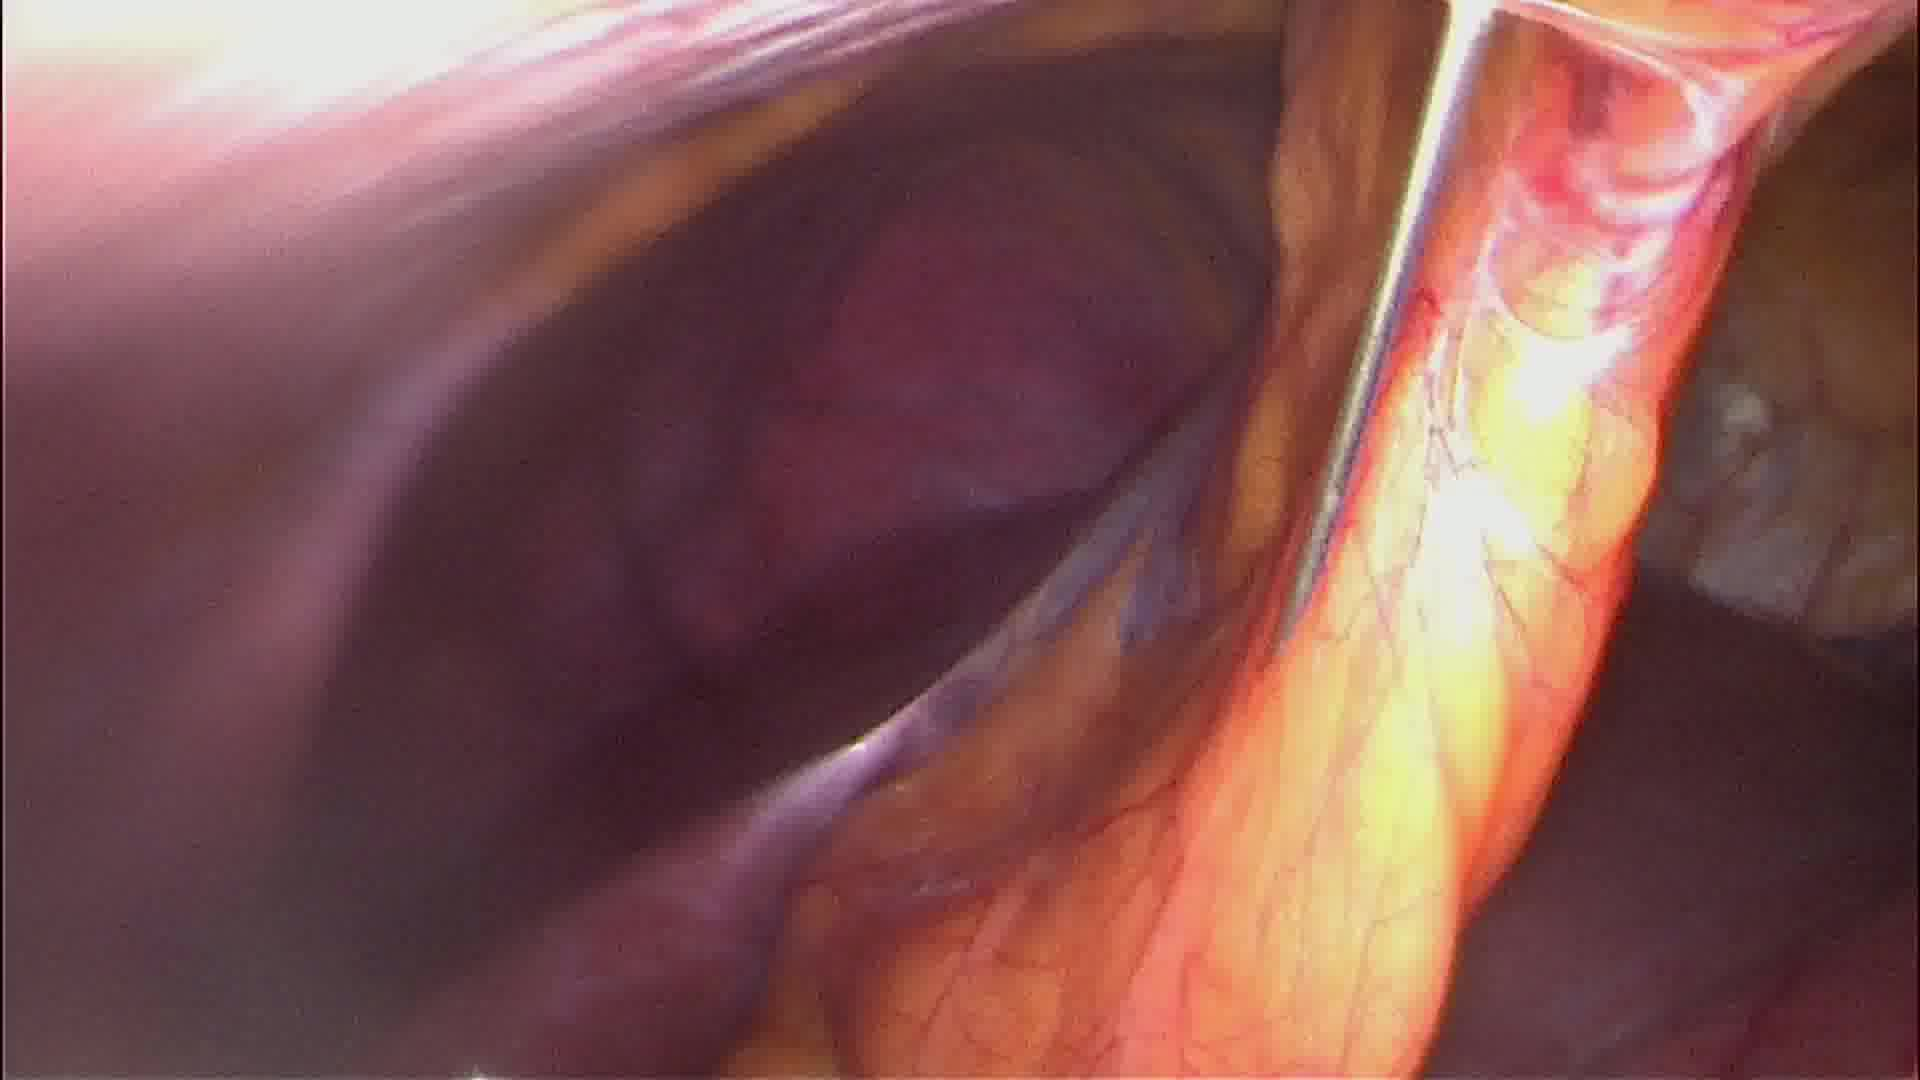
\includegraphics[width=.45\linewidth]{images/m2cai.jpg}
			%		\caption{80000 train images, 20000 test images, 101 classes}
			\label{fig:2images}
		\end{figure}
	
	Videos resolution is 1920 x 1080, shot at 25 frames per second at the IRCAD research center in Strasbourg, France.
	
	\begin{itemize}
		\item 27 training videos %(67,595 images)
		%\item 22 train videos %(59,493 images)
		%\item 5 val videos %(8,062 images)
		\item 15 test videos %(28,732 images)
		%\item 8 classes (CleaningCoagulation, CalotTriangleDissection, CLippingCutting, etc.)
	\end{itemize}
	
\end{frame}

\begin{frame}{M2CAI Workflow Dataset}

	1 of 8 classes for each frames:
	\begin{itemize}
		\item TrocarPlacement
		\item Preparation
		\item CalotTriangleDissection
       	\item ClippingCutting
       	\item GallbladderDissection
       	\item GallbladderPackaging
       	\item CleaningCoagulation
       	\item GallbladderRetraction
    \end{itemize}

\end{frame}

\begin{frame}{M2CAI Workflow Goal and Measure}
	
	  Online prediction: $P(y | x_i, x_{i-1}, x_{i-2}, ...)$  
		
		$x_i$:= frame $i$, and $y$:= classes
		
		%Detecting at which of the 8 phases of the operation each frames belong.
		
		
		Useful to:
		\begin{itemize}
			\item monitor surgeons
			\item trigger automatic actions
		\end{itemize}
		
		
		Measures:
		- Jaccard similarity coefficient:
	    $J(A,B) = \frac{| A \cap B |}{| A \cup B|} = \frac{| A \cap B |}{| A| + |B| - |A \cap B|}$
	    
	  - Accuracy top1: nb frames well classified / nb total frames
		
\end{frame}




\section{Our method} \subsection{}\label{}

\begin{frame}{Two fold}

	Training models to classify from images (frames)
	
	Extract features from CNN
	Fine tuning CNN
	
	Smoothing the predictions of our model
	
	1. averaging
	2. HMM
	
\end{frame}


\begin{frame}{1. Extracting images}

	Train
	
	Val

\end{frame}

\begin{frame}{2. Training a frame classifier}

	Features extraction
	

\end{frame}

\begin{frame}{2. Training a frame classifier}

	Fine tuning CNN
	

\end{frame}

\begin{frame}{2. Training a frame classifier}

	Fine tuning CNN with Weldon
	

\end{frame}

\begin{frame}{3. Smoothing the predictions}

	Avereging
	

\end{frame}

\begin{frame}{3. Smoothing the predictions}

	HMM online
	

\end{frame}

\begin{frame}{3. Smoothing the predictions}

	HMM offline
	

\end{frame}
	
	
\section{Experiments} \subsection{}\label{}

\begin{frame}{Validation set}
	

\end{frame}

\begin{frame}{Visualization}

	by classes	
	
\end{frame}

\begin{frame}{Visualization}

	hmm A
	
\end{frame}

\begin{frame}{Visualization}

	hmm mus
	
\end{frame}


\section{Conclusion} \subsection{}\label{}

\begin{frame}{Conclusion}

	lolz
	
\end{frame}